\documentclass[11pt]{article}
\usepackage[scaled=0.92]{helvet}
\usepackage{geometry}
\geometry{letterpaper,tmargin=1in,bmargin=1in,lmargin=1in,rmargin=1in}
\usepackage[parfill]{parskip} % Activate to begin paragraphs with an empty line rather than an indent %\usepackage{graphicx}
\usepackage{amsmath,amssymb, mathrsfs, dsfont}
\usepackage{tabularx}
\usepackage[font=footnotesize,labelfont=bf]{caption}
\usepackage{graphicx}
\usepackage{xcolor}
%\usepackage[linkbordercolor ={1 1 1} ]{hyperref}
%\usepackage[sf]{titlesec}
\usepackage{natbib}
\usepackage{../../Tianpei_Report}

%\usepackage{appendix}
%\usepackage{algorithm}
%\usepackage{algorithmic}

%\renewcommand{\algorithmicrequire}{\textbf{Input:}}
%\renewcommand{\algorithmicensure}{\textbf{Output:}}



\begin{document}
\title{Lecture 1: Hilbert Space}
\author{ Tianpei Xie}
\date{ Nov. 18th., 2022 }
\maketitle
\tableofcontents
\newpage
\section{Metric Space}
\subsection{Basics}
\begin{itemize}
\item \begin{definition}
A \emph{\textbf{metric space}} is a set $M$ and a real-valued function $d(\cdot , \cdot): M \times M \rightarrow \bR$  which satisfies:
\begin{enumerate}
\item (\emph{\textbf{Non-Negativity}}) $d(x, y) \ge 0$
\item (\emph{\textbf{Definiteness}}) $d(x, y) = 0$ if and only if $x = y$
\item (\emph{\textbf{Symmetric}}) $d(x, y) = d(y, x)$
\item (\emph{\textbf{Triangle Inequality}}) $d(x, z) \le d(x, y) + d(y, z)$
\end{enumerate} The function $d$ is called a \underline{\emph{\textbf{metric}}} on $M$. The metric space $M$ equipped with metric $d$ is denoted as $(M, d)$.
\end{definition}

\item \begin{definition} (\emph{\textbf{Cauchy Sequence}})\\
A sequence of elements $\{x_n\}$ of a metric space $(M, d)$ is called a \underline{\emph{\textbf{Cauchy sequence}}} if $\forall \epsilon >0$, there exists $N \in \bN$, for all $n, m \ge N$, $d(x_n, x_m ) < \epsilon$.
\end{definition}

\item \begin{proposition}
Any convergent sequence is a Cauchy sequence.
\end{proposition} Note that this is the direct result of \emph{triangle inequality property of a metric}.

\item \begin{definition}  (\emph{\textbf{Complete Metric Space}})\\
A metric space in which \emph{\textbf{all Cauchy sequences converge}} is called \underline{\emph{\textbf{complete}}}.
\end{definition}

\item \begin{remark}
In complete metric space, one can prove convergence \emph{without knowing what point the sequence converges to}.
\end{remark}

\item \begin{example}
The space of \emph{all absolutely integrable functions} $\cL^{1}(X, \mu)$ is \emph{\textbf{complete}}.
\end{example}

\item \begin{definition}  (\emph{\textbf{Denseness}})\\
A set $B$ in a \emph{metric space} $M$ is called \underline{\emph{\textbf{dense}}} if \emph{every $m \in M$ is a limit of elements in $B$}.
\end{definition}

\item \begin{definition} (\emph{\textbf{Continuity}})\\
A function $f: (X, d) \rightarrow (Y, p)$ is called \emph{\textbf{continuous}} at $x$ if $f(x_n) \stackrel{p}{\rightarrow} f(x)$ whenever $x_n \stackrel{d}{\rightarrow} x$.
\end{definition}

\item \begin{definition}  (\emph{\textbf{Isometry}})\\
A \emph{\textbf{bijection}} $h: (X, d) \rightarrow (Y, p)$ which \emph{\textbf{preserves} the metric}, that is,
\begin{align*}
p(h(x), h(y)) = d(x, y)
\end{align*}
is called an \underline{\emph{\textbf{isometry}}}. It is automatically \emph{continuous}. $(X, d)$ and $(Y, p)$ are said to be \emph{\textbf{isometric}} if such an isometry exists.
\end{definition}
\end{itemize}

\subsection{Equicontinuity}
\begin{itemize}
\item \begin{definition}  (\emph{\textbf{Equicontinuity}}) \citep{reed1980methods} \\
Let $\srF$ be a family of functions from a metric space $(X, p)$ to another metric space $(Y, d)$. We say $\srF$ is an \underline{\emph{\textbf{equicontinuous family}}} if and only if for all $\epsilon >0$ and all $x \in X$, there exists $\delta > 0$ such that $d(f(x), f(x')) < \epsilon$ whenever $p(x, x') < \delta$ \emph{\textbf{for every $f \in \srF$}} and all $x' \in X$.

We say $\srF$ is a \underline{\emph{\textbf{uniformly equicontinuous family}}} if and only if for all $\epsilon >0$, there exists $\delta > 0$ such that $d(f(x), f(x')) < \epsilon$ whenever $p(x, x') < \delta$ for all $x, x' \in X$ and \emph{\textbf{every $f \in \srF$}}.
\end{definition}

\item \begin{remark}
An \emph{equicontinuous family} of functions is \emph{a family of continuous functions}.
\end{remark}

\item \begin{remark}
The concept of \emph{\textbf{equicontinuity}} is with respect to \emph{\textbf{a family of functions}}, while the concept of \emph{continuity} is \emph{for one fixed function}. In other word, for continuous function $f$, the radius of input $\delta := \delta(\epsilon, x, f)$ depends on threshold $\epsilon$, the point of continuity $x$ and the function of concern $f$. But for an \emph{\textbf{equicontinuous family}}, $\delta := \delta(\epsilon, x)$ does not depends on which function $f \in \srF$. For a \emph{\textbf{uniform equicontinuous family}}, $\delta := \delta(\epsilon)$ does not depends on which function $f \in \srF$ and which point $x$ for continuity.
\end{remark}

\item \begin{remark}
We can control the behavior of $\lim\limits_{n\rightarrow \infty}f_n(x)$ in two ways \citep{reed1980methods}:
\begin{enumerate}
\item \emph{\textbf{Control its dependence on $x$}}: If the \emph{convergence} of $\{f_n(x)\}$ \emph{does not depends on the \textbf{choice of $x$}}, we have \emph{\textbf{uniform convergence}}. \emph{\textbf{Otherwise}}, we have \emph{\textbf{pointwise convergence}}.
\item  \emph{\textbf{Control its dependence on $n$}}: If the \emph{convergence} of $\{f_n(x)\}$ \emph{does not depends on \textbf{choice of function $f_n$}}, we have an \emph{\textbf{equicontinuous family $\{f_n\}$}}. This time it reveals the behavior of $x$ in the limit.  What we will see is that one can obtain not only information about the $x$ behavior of the limit but that one can also turn weak information about the approach to the limit into stronger information.
\end{enumerate}
\end{remark}

\item \begin{proposition}
Let $f_n$ be a sequence of functions from one metric space to another with the property that the family $\{f_n\}$ is \textbf{equicontinuous}. Suppose
that $f_n(x) \rightarrow f(x)$ \textbf{pointwise} for each $x$. Then $f$ is \textbf{continuous}.
\end{proposition}

\item We see that \emph{\textbf{pointwise convergence}} on a \emph{\textbf{dense set}} combined with \emph{\textbf{equicontinuity}} implies \emph{\textbf{pointwise convergence everywhere}}.
\begin{proposition} \citep{reed1980methods}\\
Let $\{f_n\}$ be an \textbf{equicontinuous family} of functions from one metric space $(X, p)$ to another $(Y, d)$ with $Y$ complete. Suppose that for a \textbf{dense} set $D \subseteq X$, we know $f_{n}(x)$ converges for all $x \in D$. Then $f_{n}(x)$ converges for all $x \in X$.
\end{proposition}

\item The following shows that uniformly equicontinuous combined with pointwise convergence implies uniform convergence.
\begin{proposition} \citep{reed1980methods}\\
Let $\{f_n\}$ be a \textbf{uniformly equicontinuous family} of functions on $[0, 1]$. Suppose that $f_n(x) \rightarrow f(x)$ for each $x$ in $[0, 1]$. Then $f_n(x) \rightarrow f(x)$  \textbf{uniformly} in $x$.
\end{proposition}

\item \begin{remark}
For functions on $[0, 1]$, \emph{every \textbf{equicontinuous family}} is \emph{\textbf{uniformly equicontinuous}}.
\end{remark}

\item \begin{theorem} (\textbf{Ascoli's Theorem}) \citep{reed1980methods}\\
Let $\{f_n\}$ be a family of \textbf{uniformly bounded equicontinuous functions} on $[0, 1]$. Then \textbf{some subsequence} $\{f_{n,m}\}$ converges \textbf{uniformly} on $[0, 1]$.
\end{theorem}
\end{itemize}

\subsection{Proof of Completeness}
\begin{itemize}
\item \begin{remark}
To prove completeness, we take an arbitrary \emph{\textbf{Cauchy sequence}} $(x_n)$ in $X$ and show that \emph{it converges in $X$}. For different spaces, such proofs may vary in complexity, but they have approximately the same general pattern:
\begin{enumerate}
\item \emph{\textbf{Construct an element $x$}} (to be used as a \emph{\textbf{limit}}).
\item \emph{\textbf{Prove that $x$ is in the space considered}}.
\item \emph{\textbf{Prove convergence $x_n \rightarrow x$} (in the sense of the \textbf{metric})}
\end{enumerate}
\end{remark}

\item \begin{proposition} (\textbf{Completeness of $\ell^{\infty}$})\\
The space $\ell^{\infty}$ is complete.
\end{proposition}
\begin{proof}
Let $(x_m)$ be any Cauchy sequence in the space  $\ell^{\infty}$, where $x_m = (\xi_1^{(m)}, \xi_2^{(m)}, \ldots)$. Since the metric on $\ell^{\infty}$ is given by
\begin{align*}
d(x, y) = \sup_{j}\abs{\xi_j - \eta_j}
\end{align*} where $x = (\xi_j)$ and $y = (\eta_j)$ and $(x_m)$ is Cauchy, for any $\epsilon > 0$ there is an $N$ such that for all $m, n > N$,
\begin{align*}
d(x_m, x_n) = \sup_{j}\abs{\xi_j^{(m)} - \xi_j^{(n)}} < \epsilon.
\end{align*}
A fortiori, for every fixed $j$,
\begin{align}
\abs{\xi_j^{(m)} - \xi_j^{(n)}} < \epsilon, \quad (m,n>N). \label{eqn: proof_l_infty_1}
\end{align}
Hence for every fixed $j$, the sequence $(\xi_j^{(1)}, \xi_j^{(2)}, \ldots)$ is a \emph{Cauchy sequence} of numbers. It converges, say, $\xi_j^{(m)} \rightarrow \xi_j$ as $m \rightarrow \infty$. Using these infinitely many limits  $\xi_1, \xi_2, \ldots,$  we define $x = (\xi_1, \xi_2, \ldots)$ and show that $x \in \ell^{\infty}$ and $x_m \rightarrow x$. From \eqref{eqn: proof_l_infty_1} with $n \rightarrow \infty$ we have
\begin{align}
\abs{\xi_j^{(m)} - \xi_j} \le \epsilon, \quad (m >N). \label{eqn: proof_l_infty_2}
\end{align}
Since $x_m = (\xi_j^{(m)}) \in \ell^{\infty}$, there is a real number $k_m$ such that $\abs{\xi_j^{(m)}} \le k_m$ for all $j$.
Hence by the triangle inequality
\begin{align*}
\abs{\xi_j} \le \abs{ \xi_j - \xi_j^{(m)}} + \abs{\xi_j^{(m)}} \le \epsilon + k_m \quad (m >N).
\end{align*}
This inequality holds for every $j$, and the right-hand side does not involve $j$. Hence $(\xi_{j})$ is a \emph{bounded} sequence of numbers. This implies
that $x = (\xi_j) \in \ell^{\infty}$.  Also, from \eqref{eqn: proof_l_infty_2} we obtain
\begin{align*}
d(x_m, x) = \sup_{j}\abs{\xi_j^{(m)} - \xi_j} \le \epsilon, \quad (m,n>N). 
\end{align*}
This shows that $x_m \rightarrow x$. Since $(x_m)$ was an arbitrary Cauchy sequence, $\ell^{\infty}$ is complete. \qed
\end{proof}

\item \begin{proposition} (\textbf{Completeness of $\cC^{0}[a,b]$})\\
The space of all continuous function under supremum norm on $[a,b]$ (, denoted as $\cC^{0}[a,b]$) is complete.
\end{proposition}
\begin{proof}
Let $(x_m)$ be any Cauchy sequence in $\cC^{0}[a, b]$. Then, given any $\epsilon > 0$, there is an $N$ such that for all $m, n> N$ we have
\begin{align}
d(x_m, x_n) = \max_{t \in J}\abs{x_m(t)  - x_n(t) } \le \epsilon  \label{eqn: c0_complete_1}
\end{align}
where $J = [a, b]$. Hence for any fixed $t = t_0 \in J$,
\begin{align*}
\abs{x_m(t_0)  - x_n(t_0) } \le \epsilon, \quad (m,n>N).
\end{align*} This shows that $(x_1(t_0), x_2(t_0), \ldots)$ is a Cauchy sequence of real numbers. Since $\bR$ is complete, the sequence converges, say,
$x_m(t_0) \rightarrow x(t_0)$ as $m \rightarrow \infty$. In this way we can associate with each $t \in J$ a unique real number $x(t)$. This defines (\emph{pointwise}) a function $x$ on $J$, and we show that $x \in \cC^{0}[a, b]$ and $x_m \rightarrow x$. From \eqref{eqn: c0_complete_1} with $n \rightarrow \infty$ we have
\begin{align*}
\max_{t \in J}\abs{x_m(t)  - x(t) } \le \epsilon, \quad (m>N).
\end{align*} Hence for every $t \in J$,
\begin{align*}
\abs{x_m(t)  - x(t) } \le \epsilon, \quad (m>N).
\end{align*} This shows that $(x_m(t))$ converges to $x(t)$ \emph{uniformly} on $J$. Since the $x_m$'s are \emph{continuous} on $J$ and the convergence is \emph{uniform}, the limit function $x$ is \emph{continuous} on $J$, as is well known from calculus. Hence $x \in \cC^{0}[a, b]$. Also $x_m \rightarrow x$. This proves completeness of $\cC^{0}[a, b]$. \qed
\end{proof}

\item \begin{theorem} (\textbf{Riesz-Fisher Theorem}) \citep{reed1980methods} \\
Let $\cL^{1}(X, \mu)$ be the space of all absolutely integrable functions on measure space $(X, \srB, \mu)$ with $\cL^1$ norm. $\cL^{1}(X, \mu)$ is complete.
\end{theorem}
\begin{proof}
Let $(f_n)$ be Cauchy sequence in $\cL^1$. It is enough to prove some \emph{\textbf{subsequence converges}} (i.e. ``\emph{Cauchy sequence in a metric space is convergent if and only if it has convergent sub-sequence}".) so pass to a subsequence (also labeled $f_n$ with $\norm{f_n - f_{n+1}}{\cL^1} \le 2^{-n}$). Let
\begin{align*}
g_m(x) = \sum_{n=1}^{m}\abs{f_n(x) - f_{n+1}(x)}
\end{align*} Let $g_{\infty}$ be the \emph{infinite sum} (which may be $\infty$). Then $g_m \le g_{m+1} \nearrow g_{\infty}$ and
\begin{align*}
\int_{X}\abs{g_m(x)}d\mu = \int_{X}\abs{\sum_{n=1}^{m}\abs{f_n(x) - f_{n+1}(x)}}d\mu \le \int_{X}\sum_{n=1}^{m}\abs{f_n(x) - f_{n+1}(x)}d\mu = \sum_{n=1}^{m}\norm{f_n - f_{n+1}}{\cL^1} \le 1,
\end{align*} so by \emph{the monotone convergence theorem}, $g_{\infty} \in \cL^1(X, \mu)$. Thus $\abs{g_{\infty}(x)} < \infty$ a.e. As a result
\begin{align*}
f_m(x) &= f_1(x) - \sum_{n=1}^{m-1}\paren{f_n(x) - f_{n+1}(x)}
\end{align*} converges pointwise a.e. to a function $f(x)$. Moreover,
\begin{align*}
\abs{f_m(x)} \le \abs{f_1(x)} + \abs{g_{\infty}(x)} < \infty
\end{align*} i.e. $f_m(x) \in \cL^1(X, \mu)$,  so $f_n \rightarrow f$ in $\cL^1$ norm by \emph{the dominated convergence theorem}. \qed
\end{proof}

\item \begin{proposition}
$\cC^{0}[a,b]$ is \textbf{dense} (w.r.t. $\norm{}{1}$) in $\cL^{1}([a,b])$. Thus $\cL^{1}([a,b])$ is the \textbf{completion} of $\cC^{0}[a,b]$ w.r.t. $\cL^1$ norm.
\end{proposition}
\end{itemize}

\newpage
\section{Hilbert Space}
\begin{itemize}
\item \begin{remark} (\emph{\textbf{Hilbert Space vs. Banach Space}})\\
Hilbert space is a special Banach space equipped with inner product. Historically, Hilbert space appears eariler.  The theory of inner product and Hilbert spaces is richer than that of general normed and Banach spaces. \emph{\textbf{Distinguishing features}} are
\begin{enumerate}
\item  \textbf{\emph{representations}} of $\cH$ as a \emph{\textbf{direct sum}} of a \emph{\textbf{closed subspace}} and its \emph{\textbf{orthogonal complement}} (section 2.3),
\item \emph{\textbf{orthonormal sets}} and sequences and corresponding \emph{\textbf{representations}} of elements of $\cH$ (section 2.5),
\item \emph{\textbf{the Riesz representation}} of \emph{\textbf{bounded linear functionals}} by inner products, (section 2.4)
\item \emph{\textbf{the Hilbert-adjoint operator}} $T^{*}$ of a bounded linear operator $T$ (section 2.10).
\end{enumerate}
\end{remark}
\end{itemize}

\subsection{Inner Product Space}
\begin{itemize}
\item \begin{remark}
Finite-dimensional vector spaces have \emph{three kinds of properties} whose generalizations we will study in the next four chapters:
\begin{enumerate}
\item \emph{\textbf{linear} properties},
\item \emph{\textbf{metric} properties}, 
\item and \emph{\textbf{geometric} properties}.
\end{enumerate}
\emph{A \textbf{Hilbert space}} generalizes the \emph{\textbf{geometric}} property of a finite-dimensional vector space to \emph{infinite-dimensional} via definition of inner product.
\end{remark}

\item \begin{definition}
A \emph{complex vector space} $V$ is called \emph{\textbf{an \underline{inner product space}}} if there is a \emph{complex-valued function} $\inn{\cdot}{\cdot}: V \times V \rightarrow \bC$ that satisfies the following four conditions for an $x, y, z \in V$ and $a,b \in \bC$:
\begin{enumerate}
\item (\textbf{\emph{Positive Definiteness}}): $\inn{x}{x} \ge 0$ and $\inn{x}{x} = 0$ if and only if $x = 0$
\item (\textbf{\emph{Linearity}}):  $\inn{a\,x + b\,y}{z} = a\inn{x}{z} + b\inn{y}{z}$ 
\item (\textbf{\emph{Hermitian}}):  $\inn{x}{y} = \overline{\inn{y}{x}}$
\end{enumerate}
The function  $\inn{\cdot}{\cdot}$  is called \emph{\textbf{an inner product}}.
\end{definition}



\item \begin{remark}
Without ``condition $\inn{x}{x} = 0$ if and only if $x = 0$", we have \emph{\textbf{semi-inner product}} \citep{conway2019course}.
\end{remark}

\item \begin{remark}
From \emph{Hermitian property}, we have $\inn{x}{a\,y + b\,z} =\overline{a}\, \inn{x}{y} + \overline{b}\, \inn{x}{z}$.
\end{remark}

\item \begin{remark}
For \emph{real vector space}, an inner product is a \emph{\textbf{symmetric covariant $2$-tensor}}, or a \emph{\textbf{symmetric bilinear form}}.
\end{remark}

\item \begin{remark}
Some books \citep{reed1980methods} define inner product via \emph{\textbf{linearity in second argument}}; while others \citep{kreyszig1989introductory, luenberger1997optimization, conway2019course} defines it in terms of \emph{\textbf{linearity in first argument}}. The difference is the position of conjugate.
\end{remark}

\item \begin{proposition}
Every \textbf{inner product space} $V$ is a \textbf{normed linear space} with the norm $\norm{x}{} = \sqrt{\inn{x}{x}}$.
\end{proposition}

\item \begin{remark}
We denote $\norm{x}{} = \sqrt{\inn{x}{x}}$ as \emph{the \textbf{length}} of a vector. With the definition of length, we can define the \emph{\textbf{distance}} $d$ as 
\begin{align*}
d(x, y) &:= \norm{x - y}{} = \sqrt{\inn{x - y}{x - y}}.
\end{align*} As a consequence of \emph{the Pythagorean Theorem}, $d$ satisfies the triangle inequality so it is a \emph{metric}. Thus \emph{\textbf{every inner product space is a metric space}}. 
\end{remark}

\item \begin{proposition} (\textbf{Parallelogram Law}) \\
For any $x, y \in (V, \inn{\cdot}{\cdot})$, 
\begin{align*}
\norm{x + y}{}^2 + \norm{x- y}{}^2 &= 2 \norm{x}{}^2 + 2\norm{y}{}^2
\end{align*}
\end{proposition}

\item \begin{remark}
The followings are other versions of \textbf{\emph{Parallelogram Law}}:
\begin{align*}
\Re \inn{x}{y} &= \frac{1}{2}\paren{\norm{x+y}{}^2 - \norm{x}{}^2 - \norm{y}{}^2}\\
\Re \inn{x}{y} &= \frac{1}{2}\paren{\norm{x}{}^2 + \norm{y}{}^2 - \norm{x-y}{}^2 }\\
\Re \inn{x}{y} &= \frac{1}{4}\paren{\norm{x+y}{}^2 - \norm{x - y}{}^2 } \\
\inn{x}{y} &= \frac{1}{4}\paren{\norm{x+y}{}^2 - \norm{x - y}{}^2 + i\norm{x+ iy}{}^2 - i \norm{x - iy}{}^2} \\
&= \Re \inn{x}{y} + i \Re \inn{x}{iy}
\end{align*}
\end{remark}

\item The converse holds true as well.
\begin{proposition}
In a \textbf{normed space} $(V, \|\cdot \|)$, if \textbf{the parallelogram law}
\begin{align*}
\norm{x + y}{}^2 + \norm{x- y}{}^2 &= 2 \norm{x}{}^2 + 2\norm{y}{}^2
\end{align*} holds, then there exists a \textbf{unique inner product} $\langle \cdot ,\ \cdot \rangle$ on $V$ such that $\norm{x}{} = \sqrt{\inn{x}{x}}$ for all $x \in V$.
\end{proposition}

\item \begin{remark}
The  inner product defines the concept of \emph{\textbf{angle}} (and \emph{orthorgonality}), and \emph{\textbf{distance}}. Hence it allows the \emph{\textbf{geometric property}} of Euclidean space to be generalized.
\end{remark}



\item \begin{definition}
Two vectors, $x$ and $y$, in an inner product space $V$ are said to be \emph{\textbf{orthogonal}} if $\inn{x}{y} = 0$. A collection $\{x_n\}$ of vectors in $V$ is called \emph{\textbf{an orthonormal set}} if $\inn{x_i}{x_i} = 1$ for all $i$, and $\inn{x_i}{x_j} = 0$ if $i\neq j$.
\end{definition}

\item \begin{theorem} (\textbf{Pythagorean Theorem})\\
Let $\{x_i\}_{i=1}^{n}$ be an \textbf{orthonormal} set in an inner product space $V$. Then for all $x \in V$,
\begin{align*}
\norm{x}{}^2 &= \sum_{i=1}^{n}\abs{\inn{x_i}{x}}^2 + \norm{x - \sum_{i=1}^{n}\inn{x_i}{x}x_i}{}^2
\end{align*}
\end{theorem}

\item \begin{corollary} (\textbf{Bessel's inequality})\\
Let $\{x_i\}_{i=1}^{n}$ be an \textbf{orthonormal} set in an inner product space $V$. Then for all $x \in V$,
\begin{align*}
\norm{x}{}^2 &\ge \sum_{i=1}^{n}\abs{\inn{x_i}{x}}^2 
\end{align*}
\end{corollary}

\item \begin{corollary} (\textbf{Cauchy-Schwartz's inequality})\\
Let $V$ be an inner product space. For $x,y \in V$,
\begin{align*}
\abs{\inn{x}{y}} &\le \norm{x}{}\,\norm{y}{}.
\end{align*}
\end{corollary}
\end{itemize}
\subsection{Hilbert Space}
\begin{itemize}
\item \begin{definition}
A \underline{\textbf{\emph{complete}}} \emph{inner product space} is called \underline{\emph{\textbf{a Hilbert space}}}. 

\emph{Inner product spaces} are sometimes called \emph{\textbf{pre-Hilbert spaces}}.
\end{definition}

\item \begin{definition}
Two Hilbert spaces $\cH_1$ and $\cH_2$ are said to be \underline{\emph{\textbf{isomorphic}}} if there is a \emph{\textbf{\underline{surjective} \underline{linear}} operator} $U: \cH_1 \rightarrow \cH_2$ such that 
\begin{align*}
\inn{Ux}{Uy}_{\cH_2} = \inn{x}{y}_{\cH_1}
\end{align*}  for all $x, y \in \cH_1$. Such an operator is called \underline{\emph{\textbf{unitary}}}.
\end{definition}

\item \begin{remark} (\emph{\textbf{Isomorphism}})\\
For vector space, an \underline{\emph{\textbf{(linear) isomorphism}}} is a \underline{\emph{\textbf{bijective linear mapping}}} from \emph{one vector spaces} to \emph{another vector space} that \emph{\textbf{preserve}} the \emph{\textbf{structure}} of that vector space. However, depending on definition of specific structure, we can have various different definition of isomorphisms:
\begin{enumerate}
\item For \underline{\emph{\textbf{metric space}}}, an \emph{isomorphism} is a \emph{bijective linear operator} that \emph{\textbf{preserves the metric}}. It is often called an \underline{\emph{\textbf{isometry}}}.
\item For \underline{\emph{\textbf{inner product space}}}, an \emph{isomorphism} is a \emph{surjective linear operator} that \emph{\textbf{preserves the inner product}}. It is often called an \underline{\emph{\textbf{surjective isometry}}}.
\item For \underline{\emph{\textbf{linear algebra}}}, an \emph{isomorphism} is a \emph{\textbf{bijective linear mapping}} that \emph{\textbf{preserves all algebraic operations}} (i.e. \emph{the vector addition} and \emph{scalar multiplication}).
\end{enumerate}

In general, \underline{\emph{\textbf{isomorphism}} is a \emph{\textbf{structure-preserving mapping}}} between two structures of the same type that \underline{\emph{can be \textbf{reversed}} by \emph{\textbf{an inverse mapping}}}. It means that ``\emph{\textbf{two spaces are essentially of the same form}}". For instance, the followings are also called \emph{\textbf{isomorphism}} depending on the context:
\begin{enumerate}
\item \emph{\textbf{homemorphism}} between \emph{topological spaces},
\item \emph{\textbf{diffeomorphism}} between \emph{smooth manifolds},
\item \emph{\textbf{bijective homomorphism}} between \emph{algebraic groups / rings / fields},
\item \emph{\textbf{graph isomorphism}} between \emph{graphs} that preseves the edge structure,
\end{enumerate}
 Also an isomorphism is called  a \emph{\textbf{transformation}} in \emph{\textbf{geometry}}, e.g. \emph{rigid transformation}, \emph{affine transformation} etc.
\end{remark}

\item \begin{example} ($\cL^2[a, b]$)\\
Define $\cL^2([a, b])$ to be the set of complex-valued measurable functions on $[a, b]$, a finite interval, that satisfy $\int_{[a, b]} \abs{f(x)}^2 dx < \infty$.
We define an inner product by
\begin{align*}
\inn{f}{g} &= \int_{a}^{b}f(x)\overline{g(x)} dx
\end{align*} $\cL^2([a, b])$ is a complete metric space. Actually, $\cL^2([a,b])$ is a completion of $\cC^{0}([a,b])$ with finite $\cL^2$ norm
\begin{align*}
\norm{f}{\cL^2} &= \paren{\int_{a}^{b} \abs{f(x)}^2 dx }^{\frac{1}{2}}
\end{align*} Thus $\cL^2([a, b])$ is a \emph{Hilbert space}.
\end{example}

\item \begin{example} ($\ell^2$)\\
Define $\ell^2$ to be \emph{the set of sequences $(x_n)_{n=1}^{\infty}$ of complex numbers} which satisfy $\sum_{n= 1}^{\infty}\abs{x_n}^2 < \infty$ with the inner product
\begin{align*}
\inn{(x_n)_{n=1}^{\infty}}{(y_n)_{n=1}^{\infty}} &= \sum_{n= 1}^{\infty}\overline{x_n}\,y_n.
\end{align*} $\ell^2$ is a complete metric space with $\ell^2$ norm 
\begin{align*}
\norm{(x_n)_{n=1}^{\infty}}{2} &= \paren{\sum_{n= 1}^{\infty}\abs{x_n}^2}^{\frac{1}{2}}.
\end{align*} So $\ell^2$ is a \emph{Hilbert space}. 

We will see that any Hilbert space that has a \emph{\textbf{countable dense set}} and is \emph{\textbf{not finite dimensional}} is \emph{\textbf{isomorphic}} to $\ell^2$ In this sense, $\ell^2$ is \emph{the canonical example} of a Hilbert space.
\end{example}

\item \begin{example} ($\cL^2(\bR^n, \mu)$)\\
Define $\mu$ to be a \emph{Borel measure} on $\bR^n$ and $\cL^2(\bR^n, \mu)$ to be the set of complex-valued measurable functions on $\bR^n$ that satisfy $\int_{\bR^n} \abs{f(x)}^2 d\mu < \infty$.
We define an inner product by
\begin{align*}
\inn{f}{g} &= \int_{\bR^n}f(x)\overline{g(x)} d\mu
\end{align*} $\cL^2(\bR^n, \mu)$ is a \emph{Hilbert space}.
\end{example}
\end{itemize}

\subsection{The Projection Theorem}
\begin{itemize}
\item \begin{remark}
\emph{\textbf{Orthogonality}} is the central concept of Hilbert space. In the presence of closed subspaces, the orthogonality allows us to decompose the Hilbert space into the direct sum of the \emph{subspace} and its \emph{orthogonal complement}.
\end{remark}

\item \begin{definition} (\emph{\textbf{Direct Sum}})\\
Suppose that $\cH_1$ and $\cH_2$ are Hilbert spaces. Then the set of \emph{pairs} $(x, y)$ with $x \in \cH_1, y \in \cH_2$ is a \emph{Hilbert space} with \emph{inner
product}
\begin{align*}
\inn{(x_1, y_1)}{(x_2, y_2)} &:= \inn{x_1}{x_2}_{\cH_1} + \inn{y_1}{y_2}_{\cH_2}
\end{align*}
This space is called \emph{\underline{\textbf{the direct sum}} of the spaces $\cH_1$ and $\cH_2$} and is denoted by $\cH_1 \oplus \cH_2$.
\end{definition}

\item \begin{definition} (\emph{\textbf{Orthogonal Complement}})\\
Let $\cM \subseteq \cH$ is a \emph{\textbf{closed}} \emph{linear subspace} of Hilbert space $\cH$ with \emph{induced inner product} $\inn{}{}$ (i.e. $\inn{x}{y}_{\cM} = \inn{x}{y}_{\cH}$ for all $x, y \in \cM$). $\cM$ is also a \emph{Hilbert space}.

We denote by $\cM^{\bot}$ the set of vectors in $\cH$ which are \emph{orthogonal} to $\cM$;  $\cM^{\bot}$ is called \emph{\textbf{the \underline{orthogonal complement} of $\cM$}}. It follows from the linearity of the inner product that $\cM^{\bot}$ is a \emph{linear subspace} of $\cH$ and an elementary argument shows that $\cM^{\bot}$ is \emph{closed}. So $\cM^{\bot}$ is also a \emph{Hilbert space}.
\end{definition}

\item \begin{remark}
The following theorem is going to show that 
\begin{align*}
\cH = \cM \oplus \cM^{\bot} = \set{x+y: x\in \cM, y \in \cM^{\bot}, \text{ i.e. }\inn{x}{y} = 0}.
\end{align*}
This important geometric property is one of the main reasons that Hilbert spaces are \emph{\textbf{easier}} to handle than Banach spaces.
\end{remark}

\item \begin{lemma}
Let $\cH$ be a Hilbert space, $\cM$ a closed subspace of $\cH$, and suppose $x \in \cH$. Then there exists in $\cM$ a \textbf{unique} element $z$ \textbf{closest} to $x$.
\end{lemma}

\begin{figure}
\begin{minipage}[t]{1\linewidth}
  \centering
  \centerline{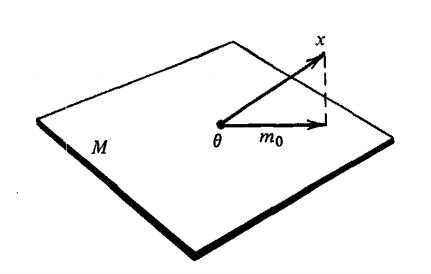
\includegraphics[scale = 0.6]{projection_theorem_hilbert.png}}
\end{minipage}
\caption{\footnotesize{\textbf{The projection theorem in Hilbert space \citep{luenberger1997optimization}}}}
\label{fig: projection_theorem_hilbert}
\end{figure}

\item \begin{theorem} (\textbf{The Projection Theorem})\\
Let $\cH$ be a Hilbert space, $\cM$ a closed subspace. Then every $x \in \cH$ can be \textbf{uniquely} written $x = z + w$ where $z \in \cM$ and $w \in \cM^{\bot}$.
\end{theorem}

\item \begin{remark}
The projection theorem sets up a natural \emph{isomorphism} $\cM \oplus \cM^{\bot} \rightarrow \cH $ given by
\begin{align*}
(z, w) \mapsto z + w
\end{align*}
We will often suppress the isomorphism and simply write $\cH = \cM \oplus \cM^{\bot}$.
\end{remark}

\end{itemize}
\subsection{The Riesz Representation Theorem}
\begin{itemize}
\item \begin{definition} (\emph{\textbf{Bounded Linear Operator}})\\
A \underline{\emph{\textbf{bounded linear transformation}}} (or \emph{\textbf{bounded operator}}) is a mapping $T: (X, \norm{\cdot}{X}) \rightarrow (Y, \norm{\cdot}{Y})$ from a normed linear space $X$ to a normed linear space $Y$ that satisfies 
\begin{enumerate}
\item (\emph{\textbf{Linearity}}) $T(\alpha x + \beta y) = \alpha T(x) + \beta T(y)$ for all $x, y \in X$, $\alpha, \beta \in \bR$ or $\bC$
\item (\emph{\textbf{Boundedness}}) $\norm{Tx}{Y} \le C\,\norm{x}{X}$ for small $C \ge 0$.
\end{enumerate} The smallest such $C$ is called \underline{\emph{the \textbf{norm} of $T$}}, written $\norm{T}{}$ or $\norm{T}{X, Y}$. Thus
\begin{align*}
\norm{T}{} &:= \sup_{\norm{x}{X} = 1 }\norm{Tx}{Y}
\end{align*}
\end{definition}

\item \begin{remark}
Denote the space of \emph{\textbf{all bounded linear operator}} between Hilbert space $\cH_1$ and $\cH_2$ as $\cL(\cH_1, \cH_2)$. The space $\cL(\cH_1, \cH_2)$ is linear space with norm 
\begin{align*}
\norm{T}{} &:= \sup_{\norm{x}{\cH_1} = 1 }\norm{Tx}{\cH_2}, \quad \forall T \in \cL(\cH_1, \cH_2).
\end{align*} It can be shown that $\cL(\cH_1, \cH_2)$ is a \emph{complete normed space (i.e. a Banach space)}.
\end{remark}

\item \begin{definition} (\emph{\textbf{Dual Space}})\\
The space $\cL(\cH, \bC)$ is called the \underline{\emph{\textbf{dual space}}} of $\cH$ and is denoted by $\cH^{*}$. The elements of $\cH^{*}$ are called \underline{\emph{\textbf{continuous linear functionals}}}. That is, the dual space $\cH^{*}$ is the space of \emph{continuous linear functionals} on $\cH$. 
\end{definition}

\item \begin{remark}
The \emph{dual space} $\cH^{*}$ is also called \emph{\textbf{covector space}} with respect to a vector space $\cH$ and the linear functionals are called \emph{\textbf{covectors}}. This terms are mostly used in \emph{differential geometry} when the vector space is \emph{the tangent space}.
\end{remark}

\item \begin{theorem} (\textbf{The Riesz Representation Theorem}) \citep{reed1980methods, kreyszig1989introductory, conway2019course} \\
For each $T \in \cH^{*}$, there is a \textbf{unique} $y_{T} \in \cH$ such that 
\begin{align*}
T(x) &= \inn{x}{y_T}
\end{align*} for all $x \in \cH$. In addition $\norm{y_{T}}{\cH} = \norm{T}{\cH^{*}}$.
\end{theorem}
\begin{proof}
Let $\cN = \text{Ker}(T) = \set{x \in \cH: T(x) = 0}$. By continuity of $T$, $\cN$ is a closed subspace of $\cH$. If $\cH = \cN$, then $T(x) = 0$ for all $x$ so for $y_T =0$, $T(x) = \inn{x}{0}$. If $\cN \subset \cH$, then there exists $x_0 \not\in \cN$. Define $y_T = \overline{T(x_0)}\frac{x_0}{\norm{x_0}{}^2}$ so for all $x = \alpha x_0$ for any $\alpha \neq 0$
\begin{align*}
T(x) = T(\alpha x_0) = \alpha T(x_0) &= \inn{\alpha x_0}{\overline{T(x_0)}\frac{x_0}{\norm{x_0}{}^2}} = \inn{x}{y_T}.
\end{align*} Note that $\cH = \text{span}\set{x_0}\oplus \cN$ since for any $x \in \cH$
\begin{align*}
x &= \paren{x - \frac{T(x)}{T(x_0)}x_0} +\frac{T(x)}{T(x_0)}x_0 \in \cN \oplus  \text{span}\set{x_0}.
\end{align*} Also $T$ and $\inn{\cdot}{y_T}$ agree on both $\cN$ and $\text{span}\set{x_0}$, so they must agree on entire $\cH$.

To prove $\norm{y_{T}}{\cH} = \norm{T}{\cH^{*}}$, we see that 
\begin{align*}
\norm{T}{\cH^{*}} &= \sup_{\norm{x}{} \le 1}\abs{Tx} =  \sup_{\norm{x}{} \le 1}\abs{\inn{x}{y_T}} \le \sup_{\norm{x}{} \le 1}\norm{x}{}\norm{y_T}{}  = \norm{y_T}{},
\end{align*} and
\begin{align*}
\norm{T}{\cH^{*}} &= \sup_{\norm{x}{} \le 1}\abs{Tx} \ge \abs{T\paren{\frac{y_T}{\norm{y_T}{}}}} = \norm{y_T}{}^{-1} \abs{\inn{y_T}{y_T}} = \norm{y_T}{}. \qed
\end{align*}
\end{proof}

\item \begin{remark}
\emph{The Riesz Representation Theorem} \citep{conway2019course, kreyszig1989introductory} is also called \emph{\textbf{The Riesz Lemma}} \citep{reed1980methods}.
\end{remark}

\item \begin{remark}
We note that \emph{the Cauchy-Schwarz inequality} shows that the \emph{\textbf{converse}} of \emph{the Riesz Representation Theorem} is \emph{\textbf{true}}. Namely, each $y \in \cH$ defines \emph{a continuous linear functional} $T_y$ on $\cH^{*}$ by
\begin{align*}
T_y(x) &= \inn{x}{y}.
\end{align*}
Thus \emph{the Riesz Representation Theorem} together with \emph{the Cauchy-Schwarz inequality} defines an \underline{\emph{\textbf{isomorphism}}  $\cH^{*} \rightarrow \cH$} between a Hilbert space $\cH$ and its dual $\cH^{*}$. In other words, unlike the case in Banach space, the bounded linear functional on Hilbert space has a simple form.
\end{remark}

\item \begin{corollary} (\textbf{The Riesz Representation for Sesquilinear Form})\\
Let $B(\cdot, \cdot)$ be a function from $\cH \times  \cH$ to $\bC$ which satisfies:
\begin{enumerate}
\item (\textbf{Linearity}) $B(\alpha x + \beta y, z) = \alpha B(x, z) + \beta B(y, z)$
\item (\textbf{Conjugate Linearity}) $B(x, \alpha y + \beta z) = \overline{\alpha} B(x, y) + \overline{\beta} B(x, z)$
\item (\textbf{Boundedness}) $\abs{B(x, y)} \le C\,\norm{x}{\cH}\,\norm{y}{\cH} $
\end{enumerate} for all $x, y, z \in \cH$, $\alpha, \beta \in \bC$. Then there is a \textbf{unique bounded linear transformation} $A: \cH \rightarrow \cH$ so that
\begin{align*}
B(x, y) = \inn{x}{Ay}
\end{align*} for all $x, y \in \cH$. The \textbf{norm} of $A$ is the smallest constant $C$ such that (3) holds.
\end{corollary}
\begin{proof}
Fix $z$, (1), (3) shows that $B(\cdot, z)$ is a continuous linear functional on $\cH$. Thus by \emph{the Riesz Representation theorem}, there exists some $y_{B,z} \in \cH$, 
\begin{align*}
B(x, z) &= \inn{x}{y_{B,z}}, \quad \forall x\in \cH
\end{align*} Define $A z = y_{B,z}$. It is not difficult to show that $A$ is a continuous linear operator with right property. \qed 
\end{proof}

\item \begin{remark}
A bilinear function on $\cH$ obeying (1) and (2) is called a \underline{\emph{\textbf{sesquilinear form}}} (as a generalization of \emph{\textbf{blinear form}} in complex vector space). 

In terms of this, an inner product in complex vector space is \emph{\textbf{a complex \underline{Hermitian form}}} (also called a \underline{\emph{\textbf{symmetric sesquilinear form}}}).
\end{remark}
\end{itemize}

\subsection{Orthonormal Bases}
\begin{itemize}
\item \begin{definition} (\emph{\textbf{Complete Orthonormal Basis}})\\
If $S$ is \emph{an orthonormal set} in a Hilbert space $\cH$ and \emph{no other orthonormal set} contains $S$ as a proper subset, then $S$ is called \emph{an \underline{\textbf{orthonormal basis}}} (or a \emph{\textbf{complete orthonormal system}}) for $\cH$.
\end{definition}

\item \begin{theorem} (\textbf{Existence of Orthonormal Basis})\\
Every Hilbert space $\cH$ has an \textbf{orthonormal basis}.
\end{theorem}

\item \begin{proposition} (\textbf{Orthogonal Representation of Element in Hilbert Space})\\
Let $\cH$ be a Hilbert space and $S = (x_{\alpha})_{\alpha \in A}$ an \textbf{orthonormal basis}. Then for each $y \in \cH$,
\begin{align}
y &= \sum_{\alpha \in A}\inn{y}{x_{\alpha}}x_{\alpha} \label{eqn: hilbert_space_orthorgonal_representation}
\end{align}
and
\begin{align}
\norm{y}{\cH} &= \sum_{\alpha \in A}\abs{\inn{y}{x_{\alpha}}}^2 \label{eqn: hilbert_space_norm_representation}
\end{align}
The equality in \eqref{eqn: hilbert_space_orthorgonal_representation} means that the sum on the right-hand side converges (independent of order) to $y$ in $\cH$. \textbf{Conversely}, if $\sum_{\alpha \in A}\abs{c_{\alpha}}^2 < \infty$,  $c_{\alpha} \in \bC$, then
$\sum_{\alpha \in A}c_{\alpha} x_{\alpha}$ converges to an element of $\cH$.
\end{proposition}

\item \begin{remark}
From Bessel's inequality, we already seen that for any finite collection $A'$ of $x_{\alpha}$, we have $\sum_{\alpha \in A'}\abs{\inn{y}{x_{\alpha}}}^2 \le \norm{y}{\cH}$. The main difficulty is on how to prove convergence of $\sum_{n=1}^{N}\abs{\inn{y}{x_{n}}}^2 $ as $N\rightarrow \infty$. Similarly we need to prove that $y-  \sum_{n=1}^{m}\inn{y}{x_{\alpha_n}}x_{\alpha_n}$ is still orthogonal to $x_{\alpha}$ as $m \rightarrow \infty$. 
\end{remark}

\item \begin{remark}
The unique coefficients $(\inn{y}{x_{\alpha}})$ is called \emph{\textbf{the Fourier coefficients of $y$} with respect to basis $(x_{\alpha})$}.
\end{remark}

\item \begin{remark} (\emph{\textbf{Gram-Schmidt Orthogonalization}})\\
Given \emph{any set of independent vectors} $(v_1, v_2, \ldots)$. we can construct \emph{an orthonormal basis} $(b_1, b_2, \ldots)$ via
\begin{align*}
b_1 &= \frac{v_1}{\norm{v_1}{}}\\
b_j &= \frac{v_j - \sum_{i=1}^{j-1}\inn{v_j}{b_i}b_i}{\norm{v_j - \sum_{i=1}^{j-1}\inn{v_j}{b_i}b_i}{}}, \quad j\ge 2
\end{align*} Thus $\text{span}\set{v_1, \xdotx{,} v_m} = \text{span}\set{b_1, \xdotx{,} b_m}$ for all $m \ge 1$.
\end{remark}
\end{itemize}
\subsection{Separability}
\begin{itemize}
\item \begin{definition} (\emph{\textbf{Separability}})\\
A \emph{metric space} which has a \underline{\emph{\textbf{countable dense subset}}} is said to be \underline{\emph{\textbf{separable}}}.
\end{definition}

\item \begin{remark}
Most Hilbert space we have seen is separable.
\end{remark}

\item \begin{proposition} (\textbf{Canonical Hilbert Space})\\
A Hilbert space $\cH$ is \textbf{separable} if and only if it has a \textbf{countable orthonormal basis} $S$. If there are $N < \infty$ elements in $S$, then $\cH$ is
\textbf{isomorphic} to $\bC^N$, If there are \textbf{countably many} elements in $S$, then $\cH$ is \textbf{isomorphic} to $\ell^{2}$.
\end{proposition}

\item \begin{remark}
Consider the map $v \mapsto (\inn{v}{x_{n}})_{n=1}^{\infty}$ for orthonormal basis $(x_n)_{n=1}^{\infty}$ as the isomorphism $\cH \rightarrow \ell^2$.
\end{remark}

\item \begin{remark}
Notice that in the separable case, \emph{the Gram-Schmidt process} anows us to construct an orthonormal basis without using \emph{Zorn's lemma}.
\end{remark}
\end{itemize}

\subsection{Fourier Series}
\begin{itemize}
\item \begin{definition}
If $f(x)$ is  integrable in $[0, 2\pi]$, define \emph{\textbf{the Fourier series}} as 
\begin{align*}
F(x) &:= \frac{1}{\sqrt{2\pi}}\sum_{n=-\infty}^{\infty}c_n e^{i n x} \\
\text{where }c_n &= \frac{1}{\sqrt{2\pi}}\int_{0}^{2\pi} e^{-i n x} f(x) dx.
\end{align*}
\end{definition}

\item \begin{proposition}
Suppose that $f(x)$ is periodic of period $2\pi$ and is continuously differentiable. Then the functions $\sum_{n=-M}^{M}c_n e^{i n x}$ converge uniformly
to $f(x)$ as $M \rightarrow \infty$.
\end{proposition}

\item \begin{proposition}
If $f \in \cL^2[0, 2\pi]$, then $\sum_{n=-M}^{M}c_n e^{i n x}$ converges to $f$ in the $\cL^2$ norm as $M \rightarrow \infty$.
\end{proposition}

\item \begin{remark}
The collection of functions, $(\frac{1}{\sqrt{2\pi}}e^{i n x})_{n=-\infty}^{\infty}$ is an \emph{\textbf{orthonormal set}} in $\cL^2[0, 2\pi]$. The above proposition states that it is a \emph{\textbf{complete} orthonormal set}, that is, for every $f \in \cL^2[0, 2\pi]$
\begin{align*}
f &= \lim\limits_{M\rightarrow \infty}\frac{1}{\sqrt{2\pi}}\sum_{n=M}^{M}c_n e^{i n x}
\end{align*}
\end{remark}
\end{itemize}

\subsection{Legendre, Hermite and Laguerre Polynomials}

\subsection{Hilbert-Adjoint Operator}
\begin{itemize}
\item \begin{definition} (\emph{\textbf{Hilbert Space Adjoint}})\\
Let $T: \cH_{1} \rightarrow \cH_{2}$ be a \emph{bounded linear operator}, where $\cH_1$ and $\cH_2$ are \emph{Hilbert spaces}. Then \underline{\emph{\textbf{the Hilbert-adjoint operator}}} $T^{*}$ of $T$ is the operator
\begin{align*}
T^{*}: \cH_2 \rightarrow \cH_1
\end{align*} such that for all $x \in \cH_1$ and $y \in \cH_2$,
\begin{align}
\inn{Tx}{y}_{\cH_2} &= \inn{x}{T^{*}y}_{\cH_1} \label{eqn: hilbert_space_adjoint}
\end{align}
\end{definition}

%\item \begin{remark}
%In general, \emph{\textbf{an adjoint operator}} is a bounded linear operator from dual space $\cH_2^{*} \rightarrow \cH_1^{*}$.
%\end{remark}

\item \begin{proposition} (\textbf{Existence of Adjoint Operator}) \citep{kreyszig1989introductory}\\
The Hilbert-adjoint operator $T^{*}$ of $T$ \textbf{exists}, is \textbf{unique} and is a \textbf{bounded linear operator} with norm
\begin{align*}
\norm{T^{*}}{} &= \norm{T}{}.
\end{align*}
\end{proposition}

\item \begin{lemma}  (\textbf{Zero operator}). \citep{kreyszig1989introductory}
Let $X$ and $Y$ be inner product spaces and $Q: X \rightarrow Y$ a bounded linear operator. Then:
\begin{enumerate}
\item $Q = 0$ if and only if $\inn{Qx}{y} = 0$ for all $x \in X$ and $y \in Y$.
\item If $Q: X \rightarrow X$, where $X$ is complex, and $\inn{Qx}{x}= 0$ for all $x \in X$, then $Q=0$.
\end{enumerate}
\end{lemma}

\item \begin{proposition} (\textbf{Properties of Hilbert-adjoint operators}).  \citep{reed1980methods, kreyszig1989introductory}\\
Let $\cH_1$, $\cH_2$ be Hilbert spaces, $S: \cH_1 \rightarrow \cH_2$ and $T: \cH_1 \rightarrow \cH_2$ bounded linear operators and $\alpha$ any scalar. Then we have
\begin{enumerate}
\item $\inn{T^{*}y}{x} = \inn{y}{Tx}$,  ($x \in H_1,  y \in \cH_2$)
\item $ (S + T)^{*} = S^{*} + T^{*}$
\item $(\alpha T)^{*} = \alpha T^{*}$
\item $(T^{*})^{*} = T$
\item $\norm{T^{*}T}{} = \norm{TT^{*}}{} = \norm{T}{}^2$
\item $T^{*}T =0 \Leftrightarrow T=0$
\item $(ST)^{*}= T^{*}S^{*}$  (assuming $\cH_2 = \cH_1$)
\item If $T$ has a \textbf{bounded inverse},  $T^{-1}$, then $T^*$ has a \textbf{bounded inverse} and $(T^{*})^{-1} = (T^{-1})^{*}$.
\end{enumerate}
\end{proposition}
\end{itemize}

\subsection{Self-Adjoint, Unitary and Normal Operators}
\begin{itemize}
\item \begin{definition}
A \textbf{\emph{bounded linear operator}} $T: \cH \rightarrow \cH$ on a Hilbert space $\cH$ is said to be
\begin{enumerate}
\item \underline{\emph{\textbf{self-adjoint}}} or \underline{\emph{\textbf{Hermitian}}} if
\begin{align*}
T^{*} = T \quad \Leftrightarrow \quad \inn{Tx}{y} = \inn{x}{Ty}
\end{align*}
\item \underline{\emph{\textbf{unitary}}} if $T$ is \emph{bijective} and
\begin{align*}
T^{*} = T^{-1} 
\end{align*}
\item \underline{\emph{\textbf{normal}}} if
\begin{align*}
T^{*}T = TT^{*}
\end{align*}
\end{enumerate}
\end{definition}

\item \begin{definition} (\emph{\textbf{Projection Operator}})\\
If $P \in \cL(\cH)$ and $P^2 = P$, then $P$ is called a \underline{\emph{\textbf{projection}}}. If in addition $P = P^*$, then $P$ is called an \underline{\emph{\textbf{orthogonal projection}}}. 
\end{definition}

\item \begin{remark}
If $T$ is \emph{\textbf{self-adjoint}} and \emph{\textbf{unitary}}, then $T$ is \emph{\textbf{normal}}.
\end{remark}

\item \begin{remark}
If a basis for $\bC^n$ is given and \emph{a \textbf{linear operator}} on $\bC^n$ is represented by a certain \emph{\textbf{matrix}}, then its \emph{\textbf{Hilbert-adjoint operator}} is represented by the \emph{\textbf{complex conjugate transpose}} of that matrix. For $\bR^n$, then the  \emph{\textbf{Hilbert-adjoint operator}} is represented by the \emph{\textbf{transpose}} of that matrix
\end{remark}

\item \begin{remark}
Similarly we have
\begin{enumerate}
\item The matrix representation for \emph{self-adjoint operator} is \emph{\textbf{Hermitian}} or \emph{\textbf{Symmetric}}. 
\begin{align*}
T^{*} = T \quad \Leftrightarrow \quad \mb{T}^{H} =\mb{T}\; (\text{ or for real vector space } \mb{T}^{T} =\mb{T})
\end{align*}
\item The matrix representation for \emph{unitary operator} is \emph{\textbf{unitary}} or \emph{\textbf{orthogonal}}. 
\begin{align*}
T^{*} = T^{-1} \quad \Leftrightarrow \quad \mb{T}^{H} =\mb{T}^{-1}\; (\text{ or for real vector space } \mb{T}^{T} =\mb{T}^{-1})
\end{align*}
\item The matrix representation for \emph{normal operator} is \emph{\textbf{normal}}. 
\begin{align*}
T^{*}T = TT^{*} \quad \Leftrightarrow \quad \mb{T}^{H}\mb{T} =\mb{T} \mb{T}^{H}\; (\text{ or for real vector space } \mb{T}^{T}\mb{T} =\mb{T} \mb{T}^{T})
\end{align*}
\end{enumerate}
\end{remark}

\item \begin{proposition} (\textbf{Self-adjointness}).  \citep{kreyszig1989introductory} \\
 Let $T: \cH \rightarrow \cH$ be a bounded linear operator on a Hilbert space $\cH$. Then:
 \begin{enumerate}
 \item If $T$ is \textbf{self-adjoint}, $\inn{Tx}{x}$ is \textbf{real} for all $x \in \cH$.
 \item If $\cH$ is complex and $\inn{Tx}{x}$ is \textbf{real} for all $x \in \cH$, the operator $T$ is\textbf{ self-adjoint}
 \end{enumerate}
\end{proposition}

\item \begin{proposition}(\textbf{Self-adjointness of product}).  \citep{kreyszig1989introductory} \\
The product of two bounded \textbf{self-adjoint} linear operators $S$ and $T$ on a Hilbert space $\cH$ is \textbf{self-adjoint} if and only if the operators \textbf{commute},
\begin{align*}
ST=TS.
\end{align*}
\end{proposition}

\item \begin{proposition} (\textbf{Sequences of self-adjoint operators}). \citep{kreyszig1989introductory}\\
 Let $(T_n)$ be a sequence of \textbf{bounded self-adjoint} linear operators $T_n: \cH \rightarrow \cH$ on a Hilbert space $\cH$. Suppose that $(T_n)$ converges, say,
 \begin{align*}
 T_n \rightarrow T, \quad \text{ i.e. } \norm{T_n - T}{} \rightarrow 0
 \end{align*}
where $\norm{\cdot}{}$ is the norm on the space $\cL(\cH, \cH)$. Then the limit operator $T$ is a \textbf{bounded self-adjoint} linear operator on $H$.
\end{proposition}

\item \begin{proposition} (\textbf{Unitary operator}). \citep{kreyszig1989introductory}\\
Let the operators $U: \cH \rightarrow \cH$ and $V: \cH \rightarrow \cH$ be \textbf{unitary}; here, $\cH$ is a Hilbert space. Then:
\begin{enumerate}
\item $U$ is \textbf{isometric}; thus $\norm{Ux}{} = \norm{x}{}$ for all $x \in \cH$;
\item $\norm{U}{}= 1$, provided $\cH \neq \{0\}$,
\item $U^{-1}= U^{*}$ is \textbf{unitary},
\item $UV$ is unitary,
\item $U$ is normal.
\item A bounded linear operator $T$ on a complex Hilbert space $\cH$ is \textbf{unitary} if and only if $T$ is \textbf{isometric} and \textbf{surjective}.
\end{enumerate}
\end{proposition}

\item \begin{remark}
Note that an \emph{\textbf{isometric operator}} need not be \emph{unitary} since it may fail to be \emph{\textbf{surjective}}. An example is the \emph{right shift operator} $T: \ell^2 \rightarrow \ell^2$ given by
\begin{align*}
(\xi_1, \xi_2, \xi_3, \ldots) \mapsto (0, \xi_1, \xi_2, \xi_3, \ldots).
\end{align*}
\end{remark}
\end{itemize}
\newpage
\bibliographystyle{plainnat}
\bibliography{reference.bib}
\end{document}